\documentclass{article}

\usepackage{amsmath}
\usepackage{amssymb}
\usepackage{bm}
\usepackage{color}
\usepackage{CJKutf8}
\usepackage{color}
\usepackage{enumitem}
\usepackage{graphicx}
\usepackage{indentfirst}
\usepackage{listings}
\usepackage{mathdots}
\usepackage{tikz}
\usepackage{wasysym}
\usepackage{xcolor}

\setlength{\parindent}{2em}

\usetikzlibrary{shapes,arrows, automata}

\allowdisplaybreaks

\newcommand{\hytt}[1]{\texttt{\hyphenchar\font=\defaulthyphenchar #1}}
\hyphenation{read-Sym-bol re-ad-Space-Tab-New-line str-Tab}

\definecolor{mygreen}{rgb}{0,0.6,0}
\definecolor{mygray}{rgb}{0.5,0.5,0.5}
\definecolor{mymauve}{rgb}{0.58,0,0.82}
%\footnotesize
\lstset{ %
  backgroundcolor=\color{white},   % choose the background color; you must add \usepackage{color} or \usepackage{xcolor}
  basicstyle=\ttfamily,            % the size of the fonts that are used for the code
  breakatwhitespace=false,         % sets if automatic breaks should only happen at whitespace
  breaklines=true,                 % sets automatic line breaking
  captionpos=b,                    % sets the caption-position to bottom
  commentstyle=\ttfamily\color{mygreen},    
                                   % comment style
  deletekeywords={},               % if you want to delete keywords from the given language
  escapeinside={},                 % if you want to add LaTeX within your code
  extendedchars=true,              % lets you use non-ASCII characters; for 8-bits encodings only, does not work with UTF-8
  frame=single,                    % adds a frame around the code
  keepspaces=true,                 % keeps spaces in text, useful for keeping indentation of code (possibly needs columns=flexible)
  keywordstyle=\color{blue},       % keyword style
  language=C++,                    % the language of the code
  morekeywords={},                 % if you want to add more keywords to the set
  numbers=left,                    % where to put the line-numbers; possible values are (none, left, right)
  numbersep=5pt,                   % how far the line-numbers are from the code
  numberstyle=\tiny\color{mygray}, % the style that is used for the line-numbers
  rulecolor=\color{black},         % if not set, the frame-color may be changed on line-breaks within not-black text (e.g. comments (green here))
  showspaces=false,                % show spaces everywhere adding particular underscores; it overrides 'showstringspaces'
  showstringspaces=false,          % underline spaces within strings only
  showtabs=false,                  % show tabs within strings adding particular underscores
  stepnumber=1,                    % the step between two line-numbers. If it's 1, each line will be numbered
  stringstyle=\color{mymauve},     % string literal style
  tabsize=2,                       % sets default tabsize to 2 spaces
  title=\lstname                   % show the filename of files included with \lstinputlisting; also try caption instead of title
}

\begin{document}
\begin{CJK*}{UTF8}{gbsn}
\CJKtilde

\title{词法分析实验报告}

\author{计算机1202 张艺瀚\\学号:20123852}
\maketitle

\section{实验题目}
词法分析

\section{实验目的}
熟悉并实现一个简单的扫描器

\section{实验内容}
\begin{enumerate}
\item 设计扫描器的自动机
\item 设计翻译、生成~\texttt{Token} 的算法
\item 编写代码并上机调试运行通过
\end{enumerate}

\section{概要设计}

本词法分析器实现扫描利用~\texttt{C++} 语言子集编写的程序,形成Token序列,建立标识符表,字符常量表和字符串常量表,在gcc 4.9.2 Ubuntu 12.04 LTS下编译通过,在测试文件下运行正常。

\texttt{LexicalAnalyzer} 类定义(代码清单~\ref{lst: classdeclarationlst})如下:
\begin{center}
\begin{lstlisting}[caption = {\texttt{LexicalAnalyzer} 类定义代码清单}, label = {lst: classdeclarationlst}]
class LexicalAnalyzer
{
public:
	LexicalAnalyzer() = default;
	LexicalAnalyzer(const string& keywordFilePath, const string& symbolFilePath);
	~LexicalAnalyzer() = default;

	void showKeywordAndSymbol();

	void LexicalAnalyze(const string& srcCodeFilePath);

	void readID(FILE* fp, char& ch);
	void readCh(FILE* fp, char& ch);
	void readStr(FILE* fp, char& ch);
	void readConst(FILE* fp, char& ch);
	void readSymbol(FILE* fp, char& ch);
	void readSpaceTabNewline(FILE* fp, char& ch);

	void showTokenSeq();
	void showIDTab();
	void showChTab();
	void showStrTab();
	void shiowConstTab();
	void showKeywordTab();
	void showSymbolTab();

private:
	vector<Token> tokenSeq;

	vector<string> idTab;
	// (0, script in idTab)

	vector<char> chTab; // dynamic
	// pay attention to \n \t \\ \' \"
	// (1, script in chTab)
	vector<string> strTab; // dynamic
	// (2, script in strTab)
	vector<double> constTab; // dynamic
	// (3, script in constTab)
	
	vector<string> keywordTab; // static
	// (script in keywordTab + 4, 0)
	// read it in readID function
	vector<string> symbolTab; // static
	// (script in symbolTab + keywordTab.size() + 4, 0)
	// read it in default condition

	Trie keywordTrie;
	Trie symbolTrie;
};
\end{lstlisting}
\end{center}

构造函数,析构函数,以~\texttt{show} 开头的输出函数此处不做详细介绍。词法分析核心功能在成员函数~\texttt{LexicalAnalyze} 中实现,其中调用了所有以~\texttt{read} 开头的读入函数,包括~\texttt{readID},~\texttt{readCh},~\texttt{readStr},~\texttt{readConst},~\texttt{readSymbol},~\texttt{readSpaceTabNewline}。下面分别介绍其设计实现。 \\

首先需要阐明关于核心内容--有限状态自动机--实现的若干考虑。利用有限状态自动机(DFA, Definite Finite Automaton)实现解析自动化和文法无关性是词法分析的核心问题。如果不考虑使用~\texttt{Lex} (或更现代的~\texttt{Flex})自动生成词法分析器,手工实现有限状态自动机的状态转换有3种常用的方式:

\begin{enumerate}
\item 使用简单的~\texttt{if-else} 语句组合。 \\
这确实是一种非常逗的方式。对于一个状态集大小为$n$,输入符集大小为$k$的DFA,它最多将包含$n*k$个转换,使用~\texttt{if-else} 描述的工作量是相当可观的,并且容易出错而不易排错。当然了,对于简单的DFA这其实是最高效的一种描述方式,~\texttt{if-else} 组合语句弱化了状态转换的概念,朴素的描述了逻辑分支,这更靠近符合程序设计者直觉的决策树。而且,可以相见,为了寥寥可数的几个状态而维护一张二维表并使用程式化的状态转化驱动程序确实有些作死了。

\item 将状态转移函数以~\texttt{switch-case} 的方式嵌入代码中。 \\
本质上这种方法与~\texttt{if-else} 实现别无二致,但形式上,~\texttt{switch-case} 对状态转换的描述要清晰得多。似乎我们为每个~\texttt{case} 赋上相应的语义动作后,DFA就跃然纸上了呢~~(当然了,这其实只欺骗自己)

\item 将状态转移函数存入状态转移矩阵(一张二维数组)中,使用程式化的DFA运行代码。 \\
这真真是极好的一种方法。它真正实现了数据与程序的分离。众所周知,组件设计应该遵循“对修改封闭,对扩展开放”的原则,对于~\texttt{if-else} 和~\texttt{switch-case} 描述方法,它们依赖于事先给定的DFA,换句话说,输入数据和处理程序是绑定的,如果状态集,输入符集或状态转换规则改变,我们不得不修改代码(这种修改常常是完全重写而非组件扩展)才能让程序正常工作,这在实际中显然是不可设想的。这时我们引入DFA这一概念已经没有意义。考虑到DFA的运行机制是统一的,不依赖于状态集,输入符集和状态转换函数,如果我们将状态转换矩阵存入一张二维表,而使用统一的驱动程序模拟DFA的运行,就将数据和处理隔离。如果状态转换改变,只需修改状态转换矩阵即可。
\end{enumerate}

另外,从文件中读入源程序的操作选择使用~\texttt{C} 风格的函数指针~\texttt{FILE*},而非~\texttt{C++} 风格的文件输入流~\texttt{ifstream}。虽然后者更加智能和强大,但它会吞掉文件中的转移字符如空格,制表符缩进,换行等,这显然会严重影响识别分析,更准确地说,这构成了对语言文法的干扰。

\subsection{\texttt{Token} 数据结构的说明}
\texttt{Token} 类定义(代码清单~\ref{lst: tokenclassdeclaration})如下:
\begin{center}
\begin{lstlisting}[caption = {\texttt{Token} 类定义代码清单}, label = {lst: tokenclassdeclaration}]
class Token
{
public:
	Token() = default;
	Token(int myType, int myVal);
	~Token() = default;

	int type;
	int val;

private:

};
\end{lstlisting}
\end{center}

其中成员变量~\texttt{type} 为类型码,成员变量~\texttt{val} 为值。~\texttt{idTab} 是用户定义的标识符列表, \texttt{chTab} 为字符常量列表,~\texttt{strTab} 为字符串常量列表,~\texttt{constTab} 为数值常量列表,~\texttt{keywordTab} 为关键字列表,~\texttt{symbolTab} 为界符列表。所有类型的~\texttt{Token} 均存放在~\texttt{Token} 列表~\texttt{tokenSeq} 中。~\texttt{idTab},~\texttt{chTab},~\texttt{strTab},~\texttt{constTab},~\texttt{tokenSeq} 为动态列表,将在词法分析的扫描过程中实时更新;~\texttt{keywordTab},~\texttt{symbolTab} 是静态列表,对于指定的程序设计语言,它们是固定的。各列表的具体结构如下表(表~\ref{tab: listtab})所示。

\begin{table}[h!]
\centering
\begin{tabular}{c|c|c}
\hline
列表&					\texttt{Token}格式&											属性 \\ \hline
\texttt{idTab}&			\texttt{(0, index in idTab)}&								动态 \\
\texttt{chTab}&			\texttt{(1, index in chTab)}&								动态 \\
\texttt{strTab}&			\texttt{(2, index in strTab)}&								动态 \\
\texttt{constTab}&		\texttt{(3, index in constTab)}&								动态 \\
\texttt{keywordTab}&		\texttt{(index in keywordTab + 4, 0)}&						静态 \\
\texttt{symbolTab}&		\texttt{(index in symbolTab + keywordTab.size() + 4, 0)}&		静态 \\
\hline
\end{tabular}
\caption{列表说明表}
\label{tab: listtab}
\end{table}

下面给出本组件所考察的~\texttt{C++} 语言子集的关键字文件~\texttt{keyword.txt} 和界符文件~\texttt{symbol.txt}。

以下为~\texttt{keyword.txt} 文件内容(代码清单~\ref{lst: keywordlst},其中第一行为关键字总数)。
\begin{center}
\begin{lstlisting}[caption = {\texttt{keyword.txt} 关键字清单}, label = {lst: keywordlst}]
22
bool
break
case
char
continue
default
do
double
else
false
float
for
if
int
long
return
short
switch
true
unsigned
void
while
\end{lstlisting}
\end{center}

以下为~\texttt{symbol.txt} 文件内容(代码清单~\ref{lst: symbollst},其中第一行为界符总数)。

注意到界符未必为字符,很多界符为字符串,更令人困扰的是它们中的一些具有公共前缀,这对词法分析的识别提出了挑战。我们当然可以为每个界符制作一部DFA进行识别,但这是相当无趣和繁冗的工作,更重要的由于公共前缀的长度是不定的,我们不能指定向前看$k$个字符来决定激活哪个DFA。当然我们可以选择手工寻找所有的公共前缀并将DFA的对应部分合并来解决这个问题,但这既繁琐又有违“输入与处理分立”的设计原则。我们将在~\texttt{readSymbol}成员函数中利用高级数据结构完美解决该问题。
\begin{center}
\begin{lstlisting}[caption = {\texttt{symbol.txt} 界符清单}, label = {lst: symbollst}]
44
(
)
[
]
{
}
+
-
*
/
++
--
=
==
+=
-=
*=
/=
>
<
>=
<=
>>
<<
>>=
<<=
&
&=
&&
|
|=
||
^
^=
!
!=
~
//
/*
*/
?
:
;
,
\end{lstlisting}
\end{center}

词法分析器将在初始化时将这些信息读入列表中。

核心成员函数~\texttt{LexicalAnalyze} 实质上是一个DFA,其中调用了所有~\texttt{read} 开头的函数,将各个读入某类字符序列的子DFA组合起来,依据当前输入符号判断将要出现的字符序列的类型,激活某一子DFA,进入对应函数,完成对改序列的读取,循环直到读入全部源文件内容,同时也完成了扫描。另外,我们规定每个函数的末尾要多读入一个字符更新当前输入符号,提供给下一个将被调用的函数使用。

\subsection{\texttt{readID} 成员函数的设计实现}
代码(代码清单~\ref{lst: readidlst})如下:
\begin{center}
\begin{lstlisting}[caption = {\texttt{readID} 成员函数代码清单}, label = {lst: readidlst}]
void LexicalAnalyzer::readID(FILE* fp, char& ch)
// automaton using if-else sentence
{
	string IDOrKeyword;
	while(isdigit(ch) || ch == '_' || isalpha(ch))
	{
		IDOrKeyword.push_back(ch);
		ch = fgetc(fp);
	}
	// cout << IDOrKeyword << endl;
	auto keywordTabPtr = find(keywordTab.begin(), keywordTab.end(), IDOrKeyword);
	auto idTabPtr = find(idTab.begin(), idTab.end(), IDOrKeyword);
	if(keywordTabPtr != keywordTab.end()) // is keyword
	{
		tokenSeq.push_back(Token(keywordTabPtr - keywordTab.begin() + 4, 0));
	}
	else // is ID
	{
		if(idTabPtr != idTab.end()) // exists in idTab
		{
			tokenSeq.push_back(Token(0, idTabPtr - idTab.begin()));
		}
		else // needs to be added to idTab
		{
			idTab.push_back(IDOrKeyword);
			tokenSeq.push_back(Token(0, idTab.size() - 1));
		}
	}
}
\end{lstlisting}
\end{center}

本函数使用~\texttt{if-else} 组合语句描述DFA,因为该DFA(如图~\ref{fig: iddfafig})形式简单。

\begin{figure}[h!]
\centering
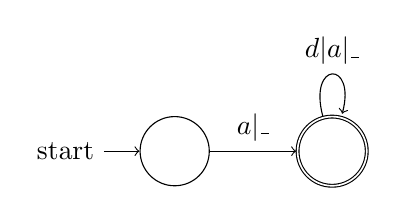
\begin{tikzpicture}[node distance = 2cm, auto]
\node[state, initial]	(q0)						{};
\node[state, accepting]	(q1)[right of = q0]		{};

\path[->]	(q0)		edge					node		{$a|\_$}		(q1)
			(q1)		edge[loop above]		node		{$d|a|\_$}	();
\end{tikzpicture}
\caption{识别标识符的DFA}
\label{fig: iddfafig}
\end{figure}

\subsection{\texttt{readCh} 成员函数的设计实现}
代码(代码清单~\ref{lst: readchlst})如下:
\begin{center}
\begin{lstlisting}[caption = {\texttt{readCh} 成员函数代码清单}, label = {lst: readchlst}]
void LexicalAnalyzer::readCh(FILE* fp, char& ch)
{
	Token token;
	token.type = 1;
	ch = fgetc(fp);
	if(ch == '\\')
	{
		char __ch__;
		__ch__ = fgetc(fp);
		switch(__ch__)
		{
			case 'n': ch = '\n'; break;
			case 't': ch = '\t'; break;
			case '\\': ch = '\\'; break;
			case '\'': ch = '\''; break;
			case '\"': ch = '\"'; break;
		}
	}

	// auto chTabPtr = find(chTab.begin(), chTab.end(), ch);
	// if(chTabPtr != chTab.end())
	// {
	// 	token.val = chTabPtr - chTab.begin();
	// 	tokenSeq.push_back(token);
	// }
	// else
	// {
	// 	chTab.push_back(ch);
	// 	token.val = chTab.size() - 1;
	// 	tokenSeq.push_back(token);
	// }

	chTab.push_back(ch);
	token.val = chTab.size() - 1;
	tokenSeq.push_back(token);

	// switch(ch)
	// {
	// 	case '\n': cout << "\\n" << endl; break;
	// 	case '\t': cout << "\\t" << endl; break;
	// 	case '\\': cout << "\\\\" << endl; break;
	// 	case '\'': cout << "\\\'" << endl; break;
	// 	case '\"': cout << "\\\"" << endl; break;
	// 	default: cout << ch << endl;
	// }

	ch = fgetc(fp);
	ch = fgetc(fp);
}
\end{lstlisting}
\end{center}
我们认为在一对单引号之间的是字符常量。

\subsection{\texttt{readStr} 成员函数的设计实现}
代码(代码清单~\ref{lst: readstrlst})如下:
\begin{center}
\begin{lstlisting}[caption = {\texttt{readStr} 成员函数代码清单}, label = {lst: readstrlst}]
void LexicalAnalyzer::readStr(FILE* fp, char& ch)
{
	string str;
	ch = fgetc(fp);
	while(ch != '\"')
	{
		if(ch == '\\')
		{
			ch = fgetc(fp);
			switch(ch)
			{
				case 'n': ch = '\n'; break;
				case 't': ch = '\t'; break;
				case '\\': ch = '\\'; break;
				case '\'': ch = '\''; break;
				case '\"': ch = '\"'; break; 
			}
		}
		str.push_back(ch);
		ch = fgetc(fp);
	}
	strTab.push_back(str);
	tokenSeq.push_back(Token(2, strTab.size() - 1));
	// cout << str << endl;
	ch = fgetc(fp);
}
\end{lstlisting}
\end{center}
我们认为,在一对双引号之间的内容是字符串常量。

\subsection{\texttt{readConst} 成员函数的设计实现}
代码(代码清单~\ref{lst: readconstlst})如下:
\begin{center}
\begin{lstlisting}[caption = {\texttt{readConst} 成员函数代码清单}, label = {lst: readconstlst}]
void LexicalAnalyzer::readConst(FILE* fp, char& ch)
// automaton whose shift function is embedded in code
{
	int state = 0;
	double d = 0.0;
	int n = 0;
	int p = 0;
	int m = 0;
	int e = 1;

	while(1)
	{
		switch(state)
		{
			// else default condition err

			case 0:
			n = 0;
			p = 0;
			m = 0;
			e = 1;
			if(isdigit(ch))
			{
				state = 1;
				n = 10 * n + (ch - '0');
			}
			else state = 9;
			break;

			case 1:
			if(isdigit(ch)) n = 10 * n + (ch - '0');
			else if(ch == 'e') state = 4;
			else if(ch == '.') state = 2;
			else state = 8;
			break;

			case 2:
			if(isdigit(ch))
			{
				state = 3;
				n = 10 * n + (ch - '0');
				++m;
			}
			else state = 9;
			break;

			case 3:
			if(isdigit(ch))
			{
				n = 10 * n + (ch - '0');
				++m;
			}
			else if(ch == 'e') state = 4;
			else state = 7;
			break;

			case 4: 
			if(ch == '-') e = -1;
			if(ch == '+' || ch == '-') state = 5;
			else if(isdigit(ch))
			{
				state = 6;
				p = 10 * p + (ch - '0');
			}
			else state = 9;
			break;

			case 5:
			if(isdigit(ch)) 
			{
				state = 6;
				p = 10 * p + (ch - '0');
			}
			else state = 9;
			break;

			case 6:
			if(isdigit(ch)) p = 10 * p + (ch - '0');
			else state = 7;
			break;

			default: break;
		}
		if(state != 7 && state != 8 && state != 9)
		{
			ch = fgetc(fp);
		}
		else
		{
			break;
		}
	}

	if(state == 9)
	{
		cerr << "Error when parsing constant!" << endl;
	}
	else
	{
		d = n * pow(10, e * p - m);
		// cout << d << endl;
		tokenSeq.push_back(Token(3, constTab.size()));
		constTab.push_back(d);
	}
}
\end{lstlisting}
\end{center}

\begin{figure}[h!]
\centering
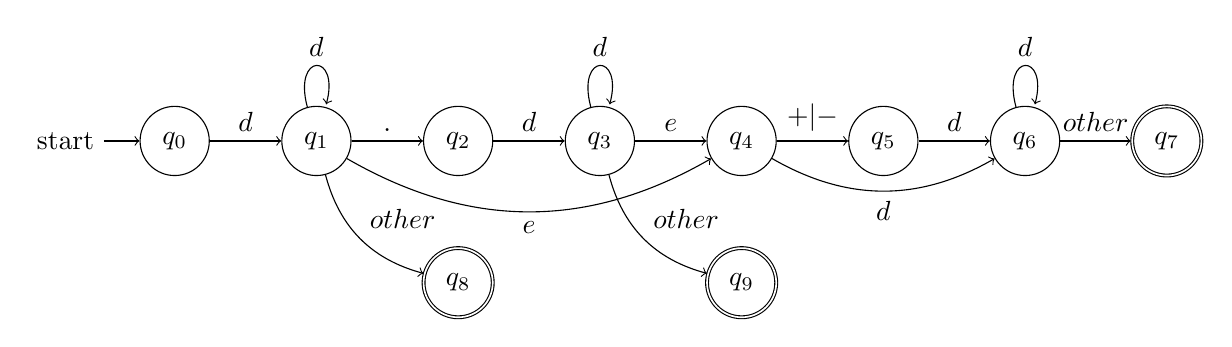
\begin{tikzpicture}[node distance = 1.8cm, auto]
\node[state, initial]	(q0)						{$q_0$};
\node[state]				(q1)[right of = q0]		{$q_1$};
\node[state]				(q2)[right of = q1]		{$q_2$};
\node[state]				(q3)[right of = q2]		{$q_3$};
\node[state]				(q4)[right of = q3]		{$q_4$};
\node[state]				(q5)[right of = q4]		{$q_5$};
\node[state]				(q6)[right of = q5]		{$q_6$};
\node[state, accepting]	(q7)[right of = q6]		{$q_7$};
\node[state, accepting]	(q8)[below of = q2]		{$q_8$};
\node[state, accepting]	(q9)[below of = q4]		{$q_9$};

\path[->]	(q0)		edge					node			{$d$}		(q1)
			(q1)		edge					node			{$.$}		(q2)
			(q2)		edge					node			{$d$}		(q3)
			(q3)		edge					node			{$e$}		(q4)
			(q4)		edge					node			{$+|-$}		(q5)
			(q5)		edge					node			{$d$}		(q6)
			(q6)		edge					node			{$other$}	(q7)
			(q1)		edge	[loop above]		node			{$d$}		()
			(q3)		edge	[loop above]		node			{$d$}		()
			(q6)		edge	[loop above]		node			{$d$}		()
			(q1)		edge	[bend right]		node[swap]	{$e$}		(q4)
			(q4)		edge	[bend right]		node[swap]	{$d$}		(q6)
			(q1)		edge	[bend right]		node			{$other$}	(q8)
			(q3)		edge	[bend right]		node			{$other$}	(q9);
\end{tikzpicture}
\caption{识别常数的DFA}
\label{fig: constdfafig}
\end{figure}

为了在扫描后不仅能够识别出常数,并且能够求出其值,我们将语义动作附加在状态上。事实上,该DFA识别正则表达式:
\[ \underbrace{\texttt{d+(.d+}}_{\text{尾数}}\texttt{(e(+|-)?}\underbrace{\texttt{d+}}_{\text{指数}}\texttt{)?)?} \]
注意到状态$q_0$和$q_1$负责扫描尾数的整数部分,$q_2$和$q_3$负责扫描尾数的小数部分,$q_6$和$q_7$负责扫描指数。根据语义容易得到下表(表~\ref{tab: semacttab})所示。

\begin{table}[h!]
\centering
\begin{tabular}{c|c}
\hline
状态&	语义动作																\\ \hline
$q_0$&		$N \leftarrow 0, p \leftarrow 0, e \leftarrow 1, m \leftarrow 0$ \\
$q_1$&		$N \leftarrow 10 \times N + [d]$ 								\\
$q_2$&		 																\\
$q_3$&		$m \leftarrow m + 1, N \leftarrow 10 \times N + [d]$ 			\\
$q_4$&		 																\\
$q_5$&		$e \leftarrow 1, if "-"$ 										\\
$q_6$&		$p \leftarrow 10 \times p + [d]$ 								\\
$q_7$&		$num \leftarrow N \times 10^{e \times p - m}$ 					\\
$q_8$&		$err$ 															\\
$q_9$&		$err$ 															\\
\hline
\end{tabular}
\caption{附加语义动作表}
\label{tab: semacttab}
\end{table}

其中$N$为不考虑小数点时的尾数值,$p$为指数值,$m$为小数点位数(自右向左)。显然有常数计算公式$num = N \times 10^{e \times p - m}$。

该函数的实现使用了前述的~\texttt{switch-case} 语句的DFA描述方式。每条~\texttt{case} 对应一个状态及附加在其上的语义动作和转移,走到终态后会得到该常数的值,效果拔群。

\subsection{\texttt{readSymbol} 成员函数的设计实现}
代码(代码清单~\ref{lst: readsymbollst})如下:
\begin{center}
\begin{lstlisting}[caption = {\texttt{readSymbol} 成员函数代码清单}, label = {lst: readsymbollst}]
void LexicalAnalyzer::readSymbol(FILE* fp, char& ch)
// use trie to replace lookahead strategy which might cause uncertainty
{
	// cout << "current character: " << ch << endl;
	symbolTrie.resetCurPtr();
	string symbol;
	while(symbolTrie.match(ch))
	{
		symbol.push_back(ch);
		ch = fgetc(fp);
	}
	tokenSeq.push_back(
		Token(find(symbolTab.begin(), symbolTab.end(), symbol) - symbolTab.begin() + keywordTab.size() + 4, 0)
		);
	// cout << "symbol identified: " << symbol << endl << endl;
}
\end{lstlisting}
\end{center}

该函数使用了吊炸天的黑科技Trie树。界符可能是一个包含多个字符的字符串,而根据~\texttt{C++} 的语法,界符与前后的词素之间不必有空格,这对于我们的识别提出了挑战,我们不容易知道界符到何处为止。当然我们可以分情况讨论,针对不同的界符适当向前看,直到可以唯一确定当前界符为止,这是一种繁冗的方法,更重要的是,我们不能预先知道到底要向前看多少个字符,只能针对具体的各个界符来讨论。当然我们也可以针对每个界符创建一个子DFA,然后在该函数中将它们并联起来,运行这个大的DFA可以做到准确识别各个界符,但这也是一种非常不优雅的方式,而且缺乏扩展性和易维护性,因为也许后期我们会扩展本扫描器所考察的语言子集,届时若需要添加所支持的界符,就必须修改代码。因此,这里我们使用字典树数据结构,它避免了盲目的向前看,我们只需要使用Trie的自带操作match,从根开始一层一层的向下匹配,直到匹配了最长的可停留在terminal属性的节点上的字符串,就得到了从该字符开始的界符。Trie的原理和在该扫描器中的实现见~\ref{sec: appendix} 附录。



\subsection{\texttt{readSpaceTabNewline} 成员函数的设计实现}
代码(代码清单~\ref{lst: readspacetabnewlinelst})如下:
\begin{center}
\begin{lstlisting}[caption = {\texttt{readSpaceTabNewline} 成员函数代码清单}, label = {lst: readspacetabnewlinelst}]
void LexicalAnalyzer::readSpaceTabNewline(FILE* fp, char& ch)
{
	while(ch == ' ' || ch == '\t' || ch == '\n')
	{
		ch = fgetc(fp);
	}
}
\end{lstlisting}
\end{center}

该函数跳过两个词素之间的所有空格,制表符和换行。

\section{源程序(包含注释)}


\section{测试数据及运行结果}
输入测试文件~\texttt{test.cpp} 内容如下(代码清单~\ref{lst: testlst})。
\begin{center}
\begin{lstlisting}[caption = {\texttt{test.txt} 关键字清单}, label = {lst: testlst}]
int f(int i)
{
	/*
	an interesting function
	*/
	++i;
	return i;
}

void g(int& i)
{
	--i;
}

int main()
{
	int x_1_x,__y22,z__123_;
	x_1_x=2*(3+(5/2)-(4<<2));
	__y22 = ~3 + (3 | 5) + (2 ^ 4) + (0 & 1);
	z__123_+=x_1_x;
	z__123_-=__y22;
	z__123_*=z__123_;
	z__123_/=z__123_;

	char _a1_       ='a';
	char b__22      = '\n';
	char __3_333___ = '\t';
	char _a_        = '\\';
	char aa         = '\'';
	char bbb        = '\"';
	char s[] = "abc\n\t\\\'\"-=~!@#$%^&*()_+";
	double d=-3.14e-10;

	bool b1=true;
	bool b2=false;
	int j=2;
	int a[10];

	// what the fuck

	for(int i=0;i<10;++i,b1=~b1,b2=b2&2)
	{
		a[i]=i;

		switch(i)
		{
			case 0:i*=2;break;
			case 1:j <<= 3; break;
			case 2:j=f(i);break;
			case 3: g(j); break;
			default:--j;break;
		}

		if(i<=5&&j!=2)
		{
			continue;
		}
		else
		{
			if(j >= 0)
			{
				b1 = false;
			}
		}
	}

	return 0;
}
\end{lstlisting}
\end{center}

\begin{center}
\begin{figure}[h!]
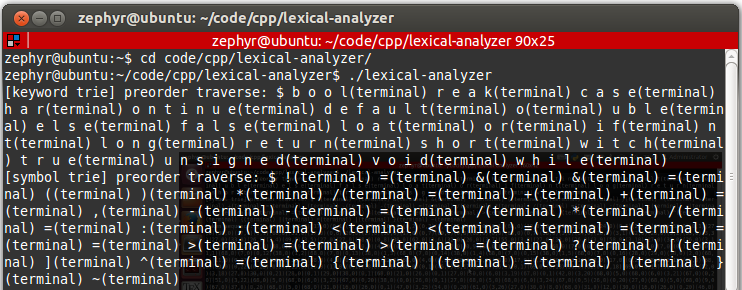
\includegraphics[width=\textwidth]{lex1.png}
\caption{运行结果截图1(keywordTrie和symbolTrie的遍历)}
\label{fig: screenshot1fig}
\end{figure}

\begin{figure}[h!]
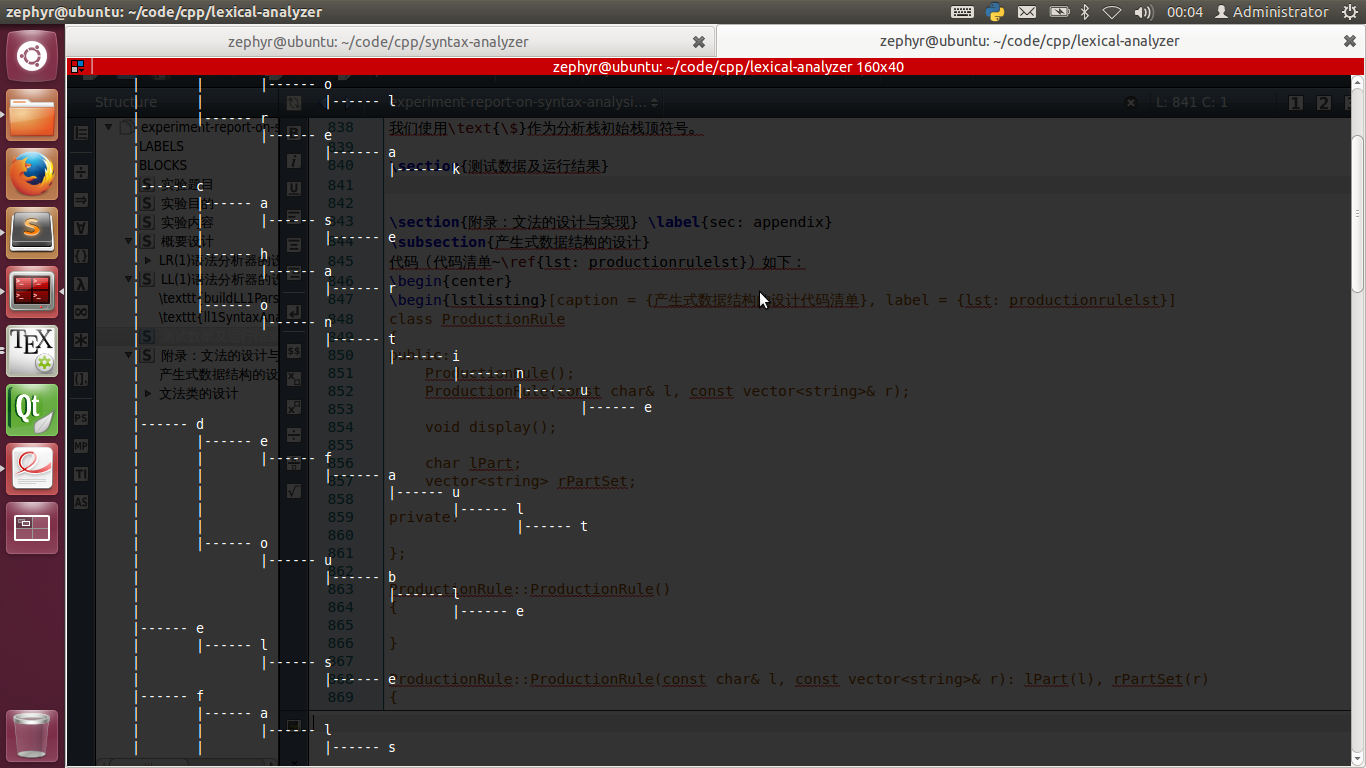
\includegraphics[width=\textwidth]{trie.png}
\caption{运行结果截图2(keywordTrie和symbolTrie的树形图谱)}
\label{fig: screenshot2fig}
\end{figure}

\begin{figure}[h!]
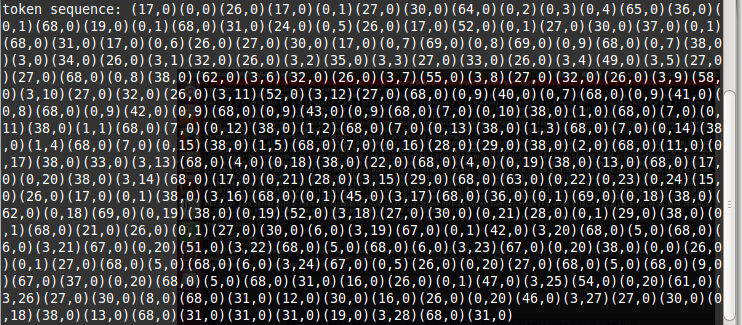
\includegraphics[width=\textwidth]{lex2.png}
\caption{运行结果截图3(Token序列)}
\label{fig: screenshot3fig}
\end{figure}

\begin{figure}[h!]
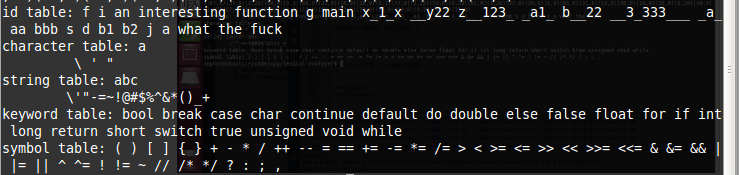
\includegraphics[width=\textwidth]{lex3.png}
\caption{运行结果截图4(标识符表,字符常量表和字符串常量表)}
\label{fig: screenshot4fig}
\end{figure}
\end{center}

\section{附录:Trie树的实现} \label{sec: appendix}

Trie即字典树,形如下图(图~\ref{fig: triefig})。

\begin{figure}[h!]
\centering
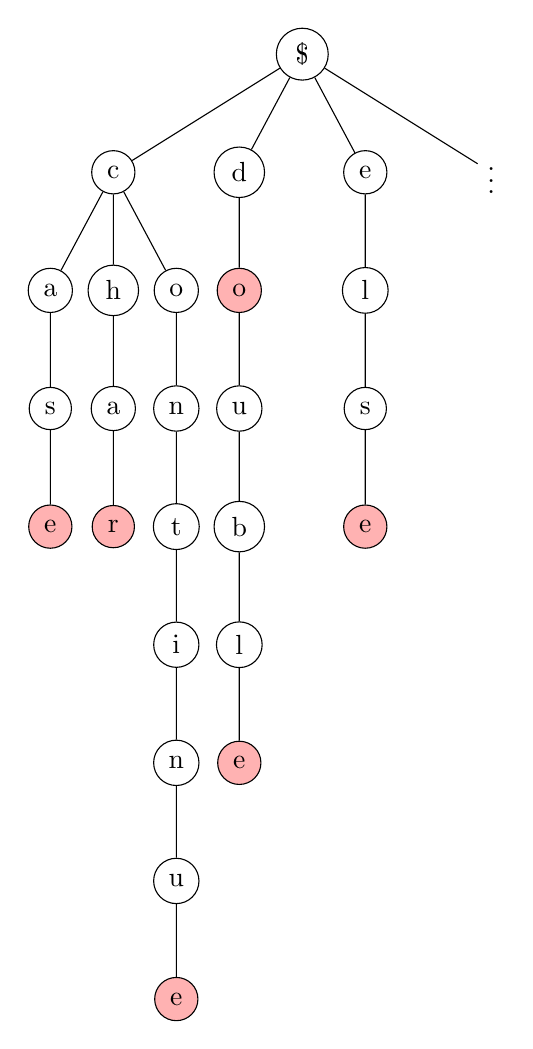
\begin{tikzpicture}
\tikzstyle{level 1} = [sibling distance = 16mm]
\tikzstyle{level 2} = [sibling distance = 8mm]
\tikzstyle{level 3} = [sibling distance = 4mm]
\node[circle, draw]{\$}
	child{node[circle, draw]{c}
		child{node[circle, draw]{a}
			child{node[circle, draw]{s}
				child{node[circle, draw, fill = red!30]{e}}}}
		child{node[circle, draw]{h}
			child{node[circle, draw]{a}
				child{node[circle, draw, fill = red!30]{r}}}}
		child{node[circle, draw]{o}
			child{node[circle, draw]{n}
				child{node[circle, draw]{t}
					child{node[circle, draw]{i}
						child{node[circle, draw]{n}
							child{node[circle, draw]{u}
								child{node[circle, draw, fill = red!30]{e}}}}}}}}}
	child{node[circle, draw]{d}
		child{node[circle, draw, fill = red!30]{o}
			child{node[circle, draw]{u}
				child{node[circle, draw]{b}
					child{node[circle, draw]{l}
						child{node[circle, draw, fill = red!30]{e}}}}}}}
	child{node[circle, draw]{e}
		child{node[circle, draw]{l}
			child{node[circle, draw]{s}
				child{node[circle, draw, fill = red!30]{e}}}}}
	child{node{$\vdots$}};
\end{tikzpicture}
\caption{Trie示意图}
\label{fig: triefig}
\end{figure}

其中红色节点表示具有terminal属性的节点,即它可以作为一个界符的尾字符。当且仅当匹配的字符串可以最终停留在terminal节点时该串才为合法界符,并且在识别中取最长合法界符。

Trie类设计如下(代码清单~\ref{lst: trielst})

\begin{center}
\begin{lstlisting}[caption = {\texttt{Trie} 类代码清单}, label = {lst: trielst}]
class Trie
{
public:
	Trie();
	~Trie();
	void destruct(Node* p);
	void insert(const string& str);
	void preorder_traverse(Node* p);
	void postorder_traverse(Node* p);
	void preorderTraverse();
	void postorderTraverse();
	void resetCurPtr();
	void preorder_traverse_display(vector<int>& stk, Node* p, bool b1);
	void display();

	bool match(char ch);

	Node* curPtr;
	Node* root;

private:

};
\end{lstlisting}
\end{center}

其中节点类~\texttt{Node} 类设计如下(代码清单~\ref{lst: nodelst})

\begin{center}
\begin{lstlisting}[caption = {\texttt{Node} 类代码清单}, label = {lst: nodelst}]
class Node
{
public:
	char val;
	vector<Node*> sons;
	bool terminal;

	Node();
	Node(const char& ch);

private:

};
\end{lstlisting}
\end{center}

每个节点包含一个值域(存放字符),一个列表(存放孩子指针)和一个属性域(标记是否为terminal)。

Trie的主要操作包括:构造,析构,前序遍历,中序遍历,后序遍历以及两个核心的附加操作为插入(\texttt{insert})和匹配(\texttt{match})。析构函数和遍历函数与一般的树相同,不再赘述,下面分别介绍构造函数, \texttt{insert} 和~\texttt{match} 成员函数的设计实现。

\subsection{构造函数的设计实现}
代码如下(代码清单~\ref{lst: constructlst})
\begin{center}
\begin{lstlisting}[caption = {构造函数代码清单}, label = {lst: constructlst}]
Trie::Trie()
{
	root = new Node('$');
	curPtr = root;
}
\end{lstlisting}
\end{center}

根节点不代表任何字符,赋予~\texttt{\$} 作为根标记。构造时只需为根节点开辟一个~\texttt{Node} 大小的空间并将根指针指向它即可即可。

\subsection{\texttt{insert} 成员函数的设计实现}
代码如下(代码清单~\ref{lst: insertlst})
\begin{center}
\begin{lstlisting}[caption = {\texttt{insert} 成员函数代码清单}, label = {lst: insertlst}]
void Trie::insert(const string& str)
{
	bool existed = false;
	Node* ptr = root;
	auto itr = str.begin();
	bool found = true;
	int mid = 0;

	while(found)
	{
		found = false;
		mid = 0;
		
		int low = 0;
		int high = ptr->sons.size() - 1;
		while(low <= high)
		{
			mid = (low + high) / 2;
			if(ptr->sons[mid]->val == *itr)
			{
				found = true;
				ptr = ptr->sons[mid];
				++itr;

				if(itr == str.end())
				{
					existed = true;
					goto next;
				}

				goto result;
			}
			else if(ptr->sons[mid]->val < *itr) low = mid + 1;
			else high = mid - 1;
		}

		result:
		if(!found)
		{
			break;
		}
	}

	next:
	if(!existed)
	{
		if(ptr->sons.empty())
		{
			mid = 0;
		}
		else if(ptr->sons[mid]->val < *itr)
		{
			++mid;
		}

		ptr->sons.insert(ptr->sons.begin() + mid, new Node(*itr));
		if(itr == str.end() - 1)
		{
			ptr->sons[mid]->terminal = true;
		}
		ptr = ptr->sons[mid];
		++itr;

		while(itr != str.end())
		{
			ptr->sons.push_back(new Node(*itr));
			if(itr == str.end() - 1)
			{
				ptr->sons[ptr->sons.size() - 1]->terminal = true;
			}
			ptr = ptr->sons[ptr->sons.size() - 1];
			++itr;
		}
	}
	else
	{
		ptr->terminal = true;
	}
}
\end{lstlisting}
\end{center}

插入过程中,我们维持孩子指针列表的有序,即另各孩子之间按字典序排列,提高访问和查询效率。在每个节点上,我们使用二分查找确定在该节点孩子指针列表的插入位置。特别的,对于以插入串的字串,仅需将这个更短的串的尾字符对应节点标记为terminal即可。

\subsection{\texttt{match} 成员函数的设计实现}
代码如下(代码清单~\ref{lst: matchlst})
\begin{center}
\begin{lstlisting}[caption = {\texttt{match} 函数代码清单}, label = {lst: matchlst}]
bool Trie::match(char ch)
{
	for(size_t i = 0; i < curPtr->sons.size(); ++i)
	{
		if(curPtr->sons[i]->val == ch)
		{
			curPtr = curPtr->sons[i];
			return true;
		}
	}
	return false;
}
\end{lstlisting}
\end{center}

该操作实现在当前节点向下匹配一个子符。在词法分析中,当且仅当待匹配串的尾字符停留在terminal节点时,匹配成功。我们预留了重置当前位置指针的接口。

\end{CJK*}
\end{document}
